%
% $RCSfile: hardware_architecture.tex,v $
%
% Copyright (C) 2002-2008. Christian Heller.
%
% Permission is granted to copy, distribute and/or modify this document
% under the terms of the GNU Free Documentation License, Version 1.1 or
% any later version published by the Free Software Foundation; with no
% Invariant Sections, with no Front-Cover Texts and with no Back-Cover
% Texts. A copy of the license is included in the section entitled
% "GNU Free Documentation License".
%
% http://www.cybop.net
% - Cybernetics Oriented Programming -
%
% http://www.resmedicinae.org
% - Information in Medicine -
%
% Version: $Revision: 1.1 $ $Date: 2008-08-19 20:41:07 $ $Author: christian $
% Authors: Christian Heller <christian.heller@tuxtax.de>
%

\subsection{Hardware Architecture}
\label{hardware_architecture_heading}
\index{Hardware Architecture}
\index{Abstract Levels of a Virtual Machine}
\index{Virtual Machine}
\index{VM}
\index{Computer Structure}
\index{Lower Levels of a Computer Structure}
\index{Higher Levels of a Computer Structure}
\index{Problem Oriented Languages}
\index{POL}

In his very clear book, Tanenbaum \cite{tanenbaum1999} organises instructions
in abstract \emph{Levels} (figure \ref{vm_figure}), which he also calls
\emph{Virtual Machines} (VM), since each level could be seen as hypothetic
computer with an own language. Further on, he considers hardware and software
to be \textit{logically equivalent} because one could replace the other.

\begin{figure}[ht]
    \begin{center}
        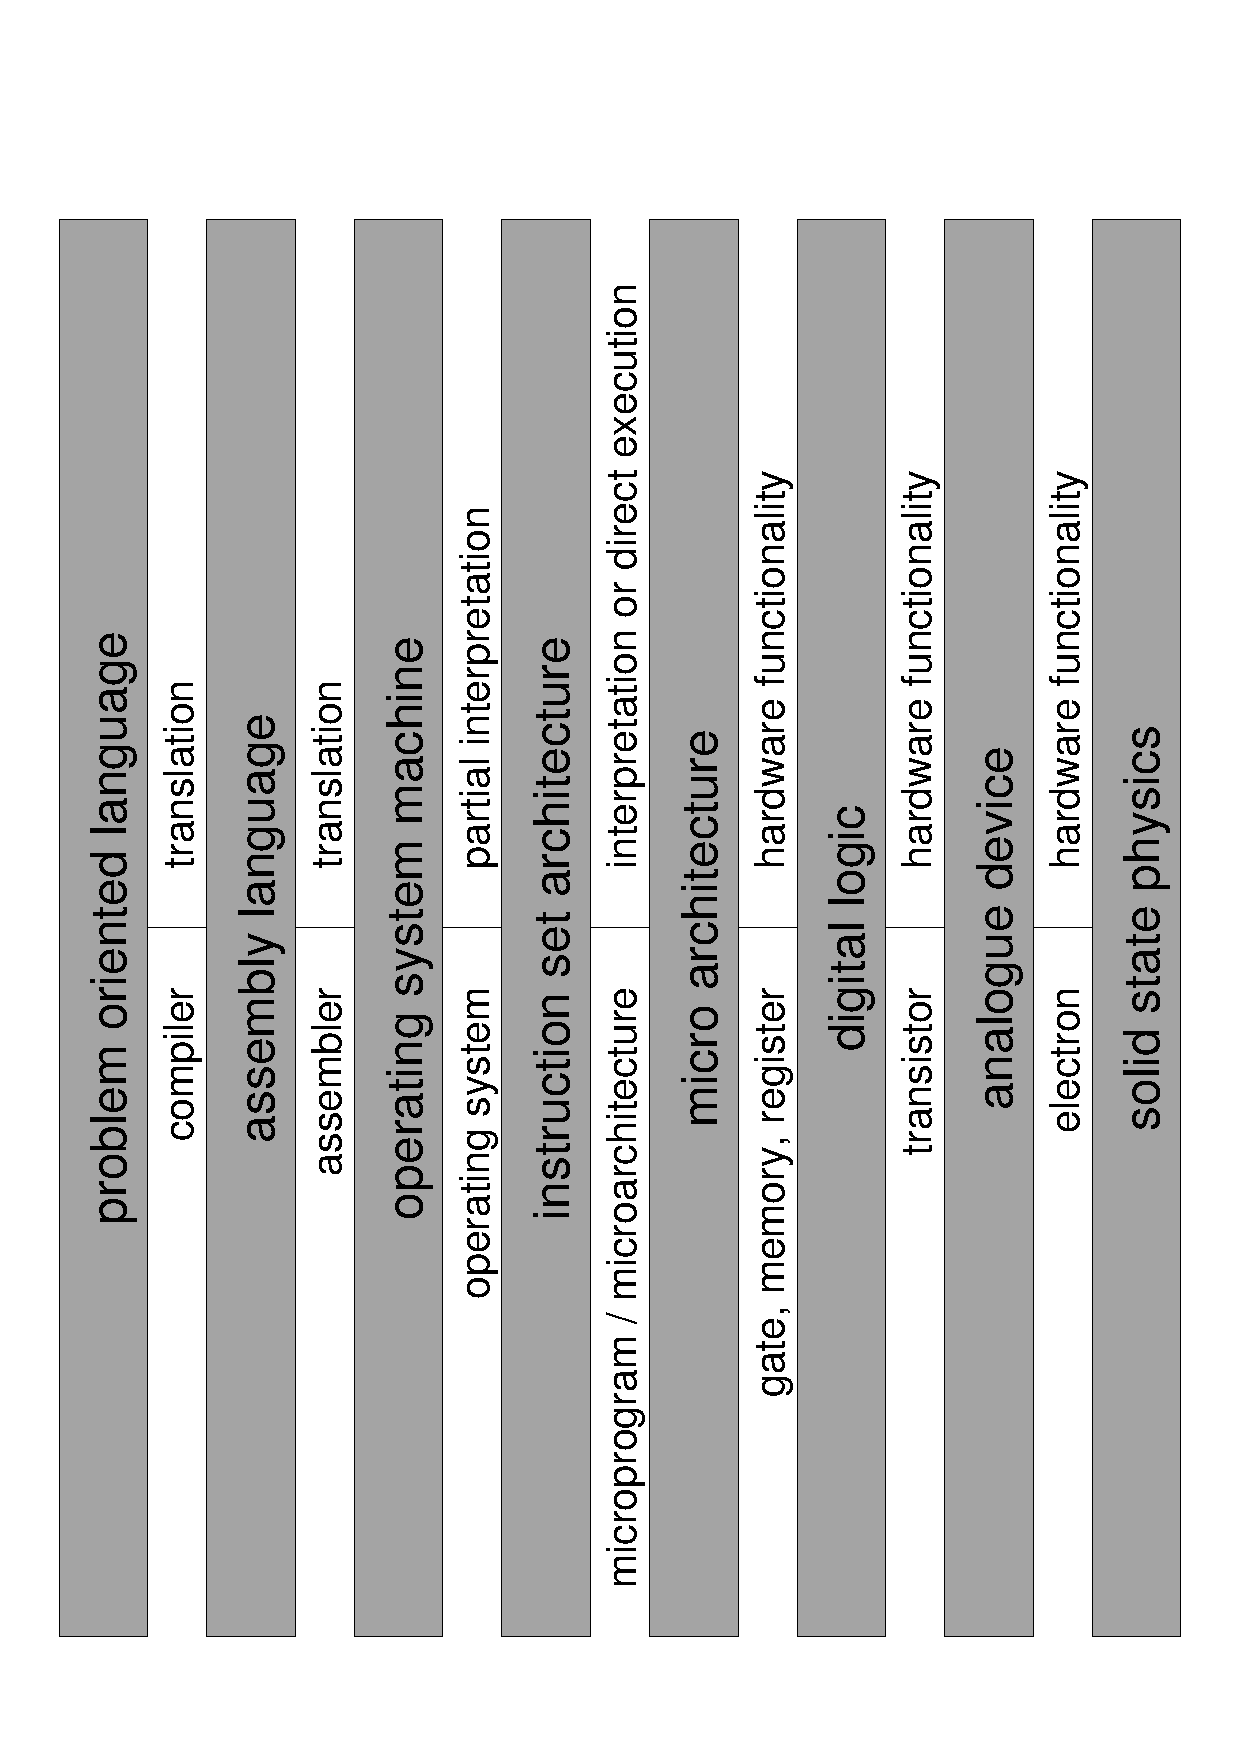
\includegraphics[scale=0.3,angle=-90]{graphic/vm.pdf}
        \caption{Computer Structure (adapted from \cite{tanenbaum1999})}
        \label{vm_figure}
    \end{center}
\end{figure}

The next sub sections are based on this structure. They describe lower levels,
close to hardware. Later sections then place more emphasis on concepts
introduced by higher-level \emph{Problem Oriented Languages} (POL).

%
% $RCSfile: digital_logic.tex,v $
%
% Copyright (C) 2002-2008. Christian Heller.
%
% Permission is granted to copy, distribute and/or modify this document
% under the terms of the GNU Free Documentation License, Version 1.1 or
% any later version published by the Free Software Foundation; with no
% Invariant Sections, with no Front-Cover Texts and with no Back-Cover
% Texts. A copy of the license is included in the section entitled
% "GNU Free Documentation License".
%
% http://www.cybop.net
% - Cybernetics Oriented Programming -
%
% http://www.resmedicinae.org
% - Information in Medicine -
%
% Version: $Revision: 1.1 $ $Date: 2008-08-19 20:41:06 $ $Author: christian $
% Authors: Christian Heller <christian.heller@tuxtax.de>
%

\subsubsection{Digital Logic}
\label{digital_logic_heading}
\index{Digital Logic}
\index{Abstract Information}
\index{States 0 and 1}
\index{Binary Digit}
\index{Bit}
\index{Gate}
\index{Logic Functions (AND, OR)}
\index{Memory}
\index{Register}
\index{Transistor}
\index{Analogue Electronic Component}
\index{Solid State Physics}
\index{Signal}
\index{Electric Voltage}
\index{Low Voltage}
\index{High Voltage}
\index{Electronic Circuit}
\index{Noise}
\index{Signal to Noise Ratio}
\index{SNR}
\index{States On and Off}
\index{States High and Low}
\index{Quantum Computer}
\index{Qubit}
\index{Elementary Particle}
\index{Spin State}
\index{Quark}

As mentioned in chapter \ref{introduction_heading}, it is \emph{Abstractions}
that enable humans to capture the surrounding real world in a simplified way.
\emph{All} information is abstract. Software is information and the data it
processes are information, too.

With the emerge of \emph{Digital Computers}, \emph{Digital Logic} gained more
importance and the new field of science \emph{Informatics} was born whose job
in essence is to break down (abstract) every piece of information to just two
states: \emph{0} and \emph{1}, represented by one \emph{Binary Digit} (Bit).
This is accomplished through the use of digital electronic components called
\emph{Gate} which transfer one or more input signals (states) into a defined
output signal by applying simple logic functions like \emph{AND} or \emph{OR}.
Many gates can form a 1-Bit \emph{Memory} that is able to store the states
\emph{0} or \emph{1}. Memories can be grouped so to form \emph{Registers}
\cite{hennessy} which are able to store one or many Bits.

Internally, gates consist of analogue electronic devices like \emph{Transistors},
the functionality of which is out of the scope of this document. Any other
details of what is going on inside analogue electronic components belong to the
field of \emph{Solid State Physics}.

One might ask why exactly \emph{0} and \emph{1} and no other states (for example
\emph{0.1}, \emph{0.2} etc.) between them were chosen. The answer needs some
background information. When talking about a \emph{Signal} in hardware computer
science, people mean electric voltage. \emph{Zero} and \emph{One} correspond to
\emph{Low} and \emph{High} voltage in electronic circuits. These minimum and
maximum values of voltage are reached in rarest cases -- mostly, the voltage lies
somewhere between. This is due to environmental influences called \emph{Noise}
which pollute a signal (voltage). Therefore, each signal has to be interpreted
as being rather high or low. The better the \emph{Signal to Noise Ratio} (SNR),
the more exact this interpretation can be.

With only two possible states, interpretation failures are very rare and digital
technique has already proven to be quite error-tolerant. How much more difficult
would it be to guess a signal's state if there were four, ten or more! That is
why breaking down all information to only \emph{High} and \emph{Low} (also
labeled \emph{True} and \emph{False} or \emph{On} and \emph{Off}) provides the
most reliable abstraction.

There are efforts to develop \emph{Quantum Computers} that use \emph{Qubits} to
measure data. While a traditional Bit represents just one state, that is either
\emph{zero} or \emph{one}, a Qubit can hold a \emph{zero}, or a \emph{one}, or
a superposition of these and represent more than one state, at one time instant.
Qubits can be implemented using elementary particles with two spin states, for
example represented by \emph{Quarks}. Quantum computers are believed to solve
certain problems faster than any classical computer \cite{wikipedia}. However,
this is the future of computing and not part of this work.

%
% $RCSfile: micro_architecture.tex,v $
%
% Copyright (C) 2002-2008. Christian Heller.
%
% Permission is granted to copy, distribute and/or modify this document
% under the terms of the GNU Free Documentation License, Version 1.1 or
% any later version published by the Free Software Foundation; with no
% Invariant Sections, with no Front-Cover Texts and with no Back-Cover
% Texts. A copy of the license is included in the section entitled
% "GNU Free Documentation License".
%
% http://www.cybop.net
% - Cybernetics Oriented Programming -
%
% http://www.resmedicinae.org
% - Information in Medicine -
%
% Version: $Revision: 1.1 $ $Date: 2008-08-19 20:41:07 $ $Author: christian $
% Authors: Christian Heller <christian.heller@tuxtax.de>
%

\subsubsection{Micro Architecture}
\label{micro_architecture_heading}
\index{Micro Architecture}
\index{Arithmetic Logic Unit}
\index{ALU}
\index{Integrated Circuit}
\index{IC}
\index{Data Path}
\index{Micro Program}
\index{Instruction Set Architecture}
\index{ISA}

The \emph{Micro Architecture} level contains a number of memories and the so
called \emph{Arithmetic Logic Unit} (ALU) which is an \emph{Integrated Circuit}
(IC) that is able to execute simple arithmetic operations. The arithmetic logic
unit and registers exchange data across the \emph{Data Path}. The data path is
controlled either directly by hardware or by a special \emph{Micro Program}
which interprets instructions from the next higher
\emph{Instruction Set Architecture} (ISA) level.

%
% $RCSfile: instruction_set_architecture.tex,v $
%
% Copyright (C) 2002-2008. Christian Heller.
%
% Permission is granted to copy, distribute and/or modify this document
% under the terms of the GNU Free Documentation License, Version 1.1 or
% any later version published by the Free Software Foundation; with no
% Invariant Sections, with no Front-Cover Texts and with no Back-Cover
% Texts. A copy of the license is included in the section entitled
% "GNU Free Documentation License".
%
% http://www.cybop.net
% - Cybernetics Oriented Programming -
%
% http://www.resmedicinae.org
% - Information in Medicine -
%
% Version: $Revision: 1.1 $ $Date: 2008-08-19 20:41:07 $ $Author: christian $
% Authors: Christian Heller <christian.heller@tuxtax.de>
%

\subsubsection{Instruction Set Architecture}
\label{instruction_set_architecture_heading}
\index{Instruction Set Architecture}
\index{ISA}
\index{Micro Architecture Hardware}
\index{Micro Program Software}

The \emph{Instruction Set Architecture} (ISA) essentially summarises the
instructions that can be carried out by the micro architecture hardware (or
interpreted by its micro program software). Computer manufacturers usually
publish a handbook describing the whole set of instructions.

